\documentclass[12pt]{article}
\usepackage[top=0.9in, bottom=0.9in, left=0.9in, right=1.1in]{geometry}

\usepackage{graphicx,color,enumitem}
\usepackage{amsmath,amsthm,amsbsy}
\usepackage{palatino}

\usepackage{tikz}

%% Setup aproblem environment, 
%% aproblem items
%% subproblems environment
%% subproblem items
\makeatletter
\newcounter{probcount}
\newcounter{subprobcount}
\newlength\probsep
\newlength\pshrinking
\newif\iffirstprob

\newenvironment{aproblems}%
  {\ifhmode\unskip\par\fi\setcounter{probcount}{0}\probsep\parskip
  \sbox\@tempboxa{\textbf{9.}}\pshrinking\wd\@tempboxa\advance\pshrinking\labelsep
  \let\hproblem\aproblem
  \advance\linewidth -\pshrinking
  \advance\@totalleftmargin\pshrinking
  \advance\leftskip\pshrinking}%
  {\ifhmode\unskip \par\fi\advance\leftskip-\pshrinking}%

\newcommand{\aproblem}{%
  \setcounter{subprobcount}{0}%
  \stepcounter{probcount}%
  \def\@currentlabel{\arabic{probcount}}%
  \ifhmode
    \unskip \par
  \fi
%  \addpenalty{-4000}%
  \iffirstprob\else\addvspace\probsep\fi
  \firstprobfalse
  \hskip -\labelwidth\hskip -\labelsep 
  \hbox to\labelwidth{\hss\textbf{\arabic{probcount}.}}\hskip\labelsep
}%


%% The following commands put defined left and right headers on the top, and a page number
%% on the bottom of all pages beyond page 1
\usepackage{fancyhdr}
\pagestyle{fancy}
\fancyfoot[C]{\ifnum \value{page} > 1\relax\thepage\fi}
\fancyhead[L]{\ifx\@doclabel\@empty\else\@doclabel\fi}
\fancyhead[R]{\ifx\@docdate\@empty\else\@docdate\fi}
\headheight 15pt
\def\doclabel#1{\gdef\@doclabel{#1}}
\def\docdate#1{\gdef\@docdate{#1}}
\makeatother

%% General formatting parameters
\parindent 0pt
\parskip 6pt plus 1pt


\doclabel{Math F251: Another Section 5.4 and 5.5 Worksheet}
\docdate{Monday 22 April 2019}


\begin{document}
\renewcommand{\d}{\displaystyle}

\begin{center}
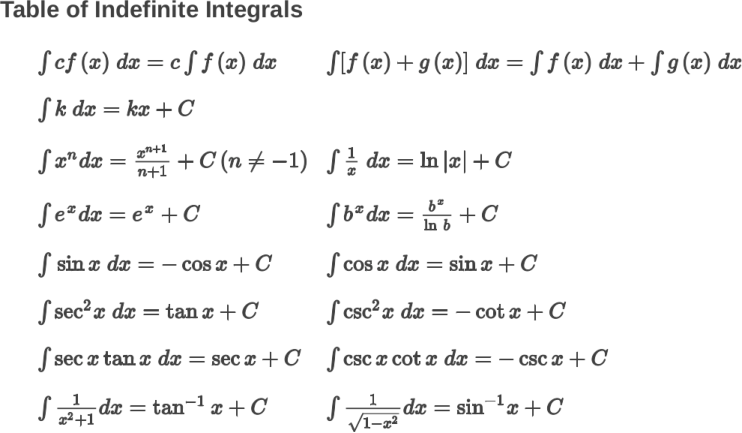
\includegraphics[width=0.65\textwidth]{inttable}
\end{center}

\vspace{-5mm}
\hrulefill

% pi trivial
% 5.4 # 31,like 34(indef),41(indef),44
% 5.5 # 50, 51, 69, 43, 26
\begin{aproblems}
\aproblem For the following integrals, decide if you would use a $u$-substitution.  If so, \emph{just write down the $u$-substitution}.  If not, \emph{evaluate the integral}.
\renewcommand{\labelenumi}{\textbf{(\alph{enumi})}}
\begin{enumerate}
\item $\d \int e^{\cos x}\sin x\,dx = $
\vfill
\item $\d \int \frac{dx}{ax+b} = $
\vfill
\item $\d \int_0^2 |2x-1| \,dx = $
\vfill
\item $\d \int_e^{e^4} \frac{dx}{x\sqrt{\ln x}} = $
\vfill
\item $\d \int (7x - 7^{-x})\,dx = $
\vfill
\item $\d \int_0^1 x(\sqrt[3]{x} + \sqrt[4]{x}) \,dx = $
\vfill
\item $\d \int \pi\,dt = $
\vfill
\item $\d \int \frac{3\,dr}{\sqrt{1-r^2}} = $
\vfill
\item $\d \int \tan^2\theta \sec^2\theta\,d\theta = $
\vfill
\item $\d \int \frac{dx}{(1+x^2)\tan^{-1}(x)} = $
\vfill
\end{enumerate}

\newpage
\thispagestyle{plain}
\aproblem Complete the $u$-substitution, or any other work, for the integrals from problem \textbf{1.}

\vspace{-20mm}
\renewcommand{\labelenumi}{\textbf{(\alph{enumi})}}
\begin{enumerate}
\item
\vfill

\item
\vfill

\item
\vfill

\item
\vfill

\item
\vfill

\item
\vfill

\item
\vfill

\item
\vfill

\item
\vfill

\item
\vfill

\end{enumerate}
\vfill

\end{aproblems}

\end{document}
